\newpage
\thispagestyle{empty}
%
\begin{spacing}{1.3}
%
\chapter{Results and Achievements}

This chapter summarizes the outcomes of the GramaGIS project and highlights the major technical, architectural, and administrative achievements accomplished during the development of this intelligent Panchayat management system.

\section{Objective 1: Spatial Digitization of Village Assets}

Village infrastructure such as ward boundaries, roads, schools, and hospitals were successfully digitized and stored in standardized geospatial formats. \cite{fu2020webgis}.

\begin{itemize}
    \item \textbf{Standardized Digital Records:} Infrastructure data was digitized from physical records and converted into OGC-compliant formats using the WGS 84 (EPSG:4326) coordinate system \cite{smart_panchayat2023}.
    \item \textbf{Layer Organization:} Multiple spatial layers including wards, roads, health centers, and educational institutions were structured for efficient visualization and analysis.
\end{itemize}

\section{Objective 2: Centralized Spatial Database using PostGIS}

A centralized spatial data infrastructure was implemented to store and manage all Panchayat datasets.

\begin{itemize}
    \item \textbf{PostGIS Spatial Database:} A relational spatial database was developed to store village datasets with spatial attributes \cite{postgis_in_action}.
    \item \textbf{Optimized Database Performance:} Implementation of \textbf{GiST-based spatial indexing} enabled fast spatial queries such as intersection and proximity searches.
\end{itemize}

\section{Objective 3: Web-based GIS Visualization}

An interactive web GIS platform was developed to visualize Panchayat infrastructure data.

\begin{itemize}
    \item \textbf{Interactive Map Interface:} A dynamic web map was implemented using Leaflet.js, enabling users to explore and filter village layers in real time.
    \item \textbf{Service Integration:} GeoServer successfully published spatial layers using WMS and WFS services for web-based access.
\end{itemize}

\section{Objective 4: Natural Language Query Interface}

The system integrates artificial intelligence to simplify spatial queries for non-technical users.

\begin{itemize}
    \item \textbf{NL2CQL Translation:} Integration of the \textbf{Gemini AI API} enabled translation of natural language queries into GeoServer \textbf{CQL\_FILTER} expressions \cite{liu2025nalspatial}.
    \item \textbf{Dynamic Map Filtering:} AI-generated filters were integrated with WMS requests, allowing maps to update dynamically based on user queries.
    \item \textbf{Usability Impact:} Panchayat staff were able to retrieve spatial information (e.g., “Show all hospitals in Ward 5”) without requiring GIS expertise.
\end{itemize}



\section{Conclusion Impact}

GramaGIS establishes a scalable geospatial framework that modernizes traditional Panchayat record management. By integrating \textbf{PostGIS}, \textbf{GeoServer}, \textbf{Leaflet}, and \textbf{Gemini AI}, the system provides an accessible and intelligent platform for spatial data management and decision support in rural governance.

\section{System Screenshots}

This section presents visual evidence of the implemented GramaGIS platform, showcasing the user interface, administrative features, and interactive capabilities.

\subsection{Landing Page Interface}

\begin{figure}[H]
    \centering
    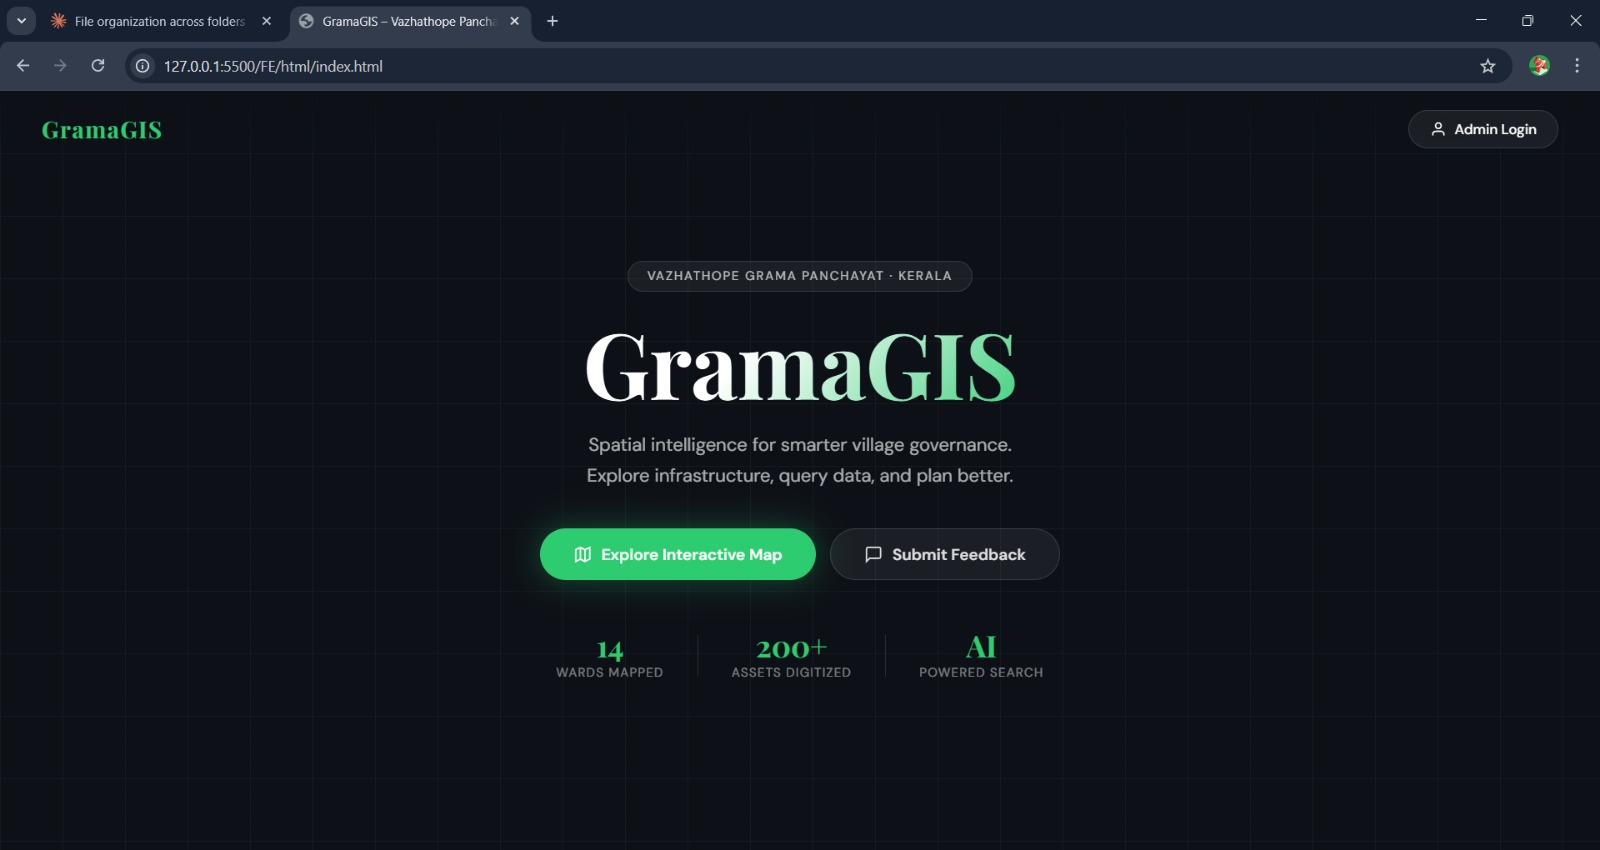
\includegraphics[width=0.85\textwidth]{Project_Screenshots/Home.jpeg}
    \caption{GramaGIS Landing Page displaying village statistics and primary navigation options}
    \label{fig:homepage}
\end{figure}

Figure \ref{fig:homepage} shows the main entry point of the GramaGIS portal. The landing page provides users with an overview of the Panchayat's digitized infrastructure, including the total number of wards mapped, assets digitized, and the AI-powered search functionality. The clean, modern interface ensures accessibility for both technical and non-technical users.

\subsection{Interactive Geospatial Map}

\begin{figure}[H]
    \centering
    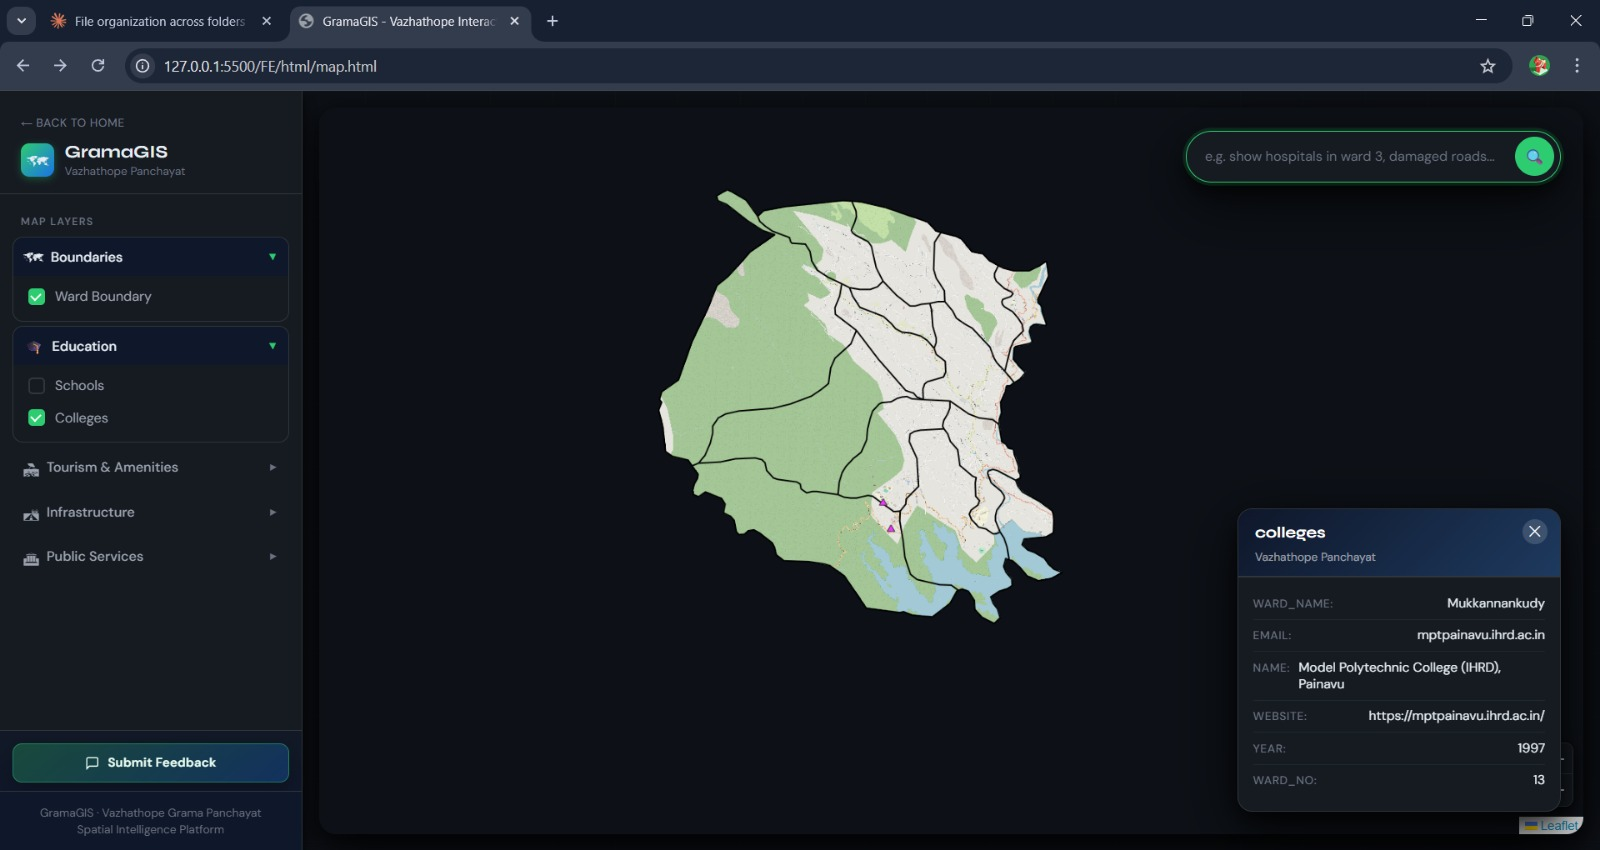
\includegraphics[width=0.95\textwidth]{Project_Screenshots/map.jpeg}
    \caption{Interactive map interface with layer controls, spatial querying, and metadata popups}
    \label{fig:map_interface}
\end{figure}

Figure \ref{fig:map_interface} demonstrates the core functionality of GramaGIS—the interactive web map powered by Leaflet.js and GeoServer. Users can toggle between different infrastructure layers (boundaries, education, healthcare, infrastructure), visualize spatial relationships, and retrieve detailed metadata by clicking on map features. The left sidebar provides hierarchical layer controls, while the search bar enables natural language queries.

\subsection{Administrator Login Portal}

\begin{figure}[H]
    \centering
    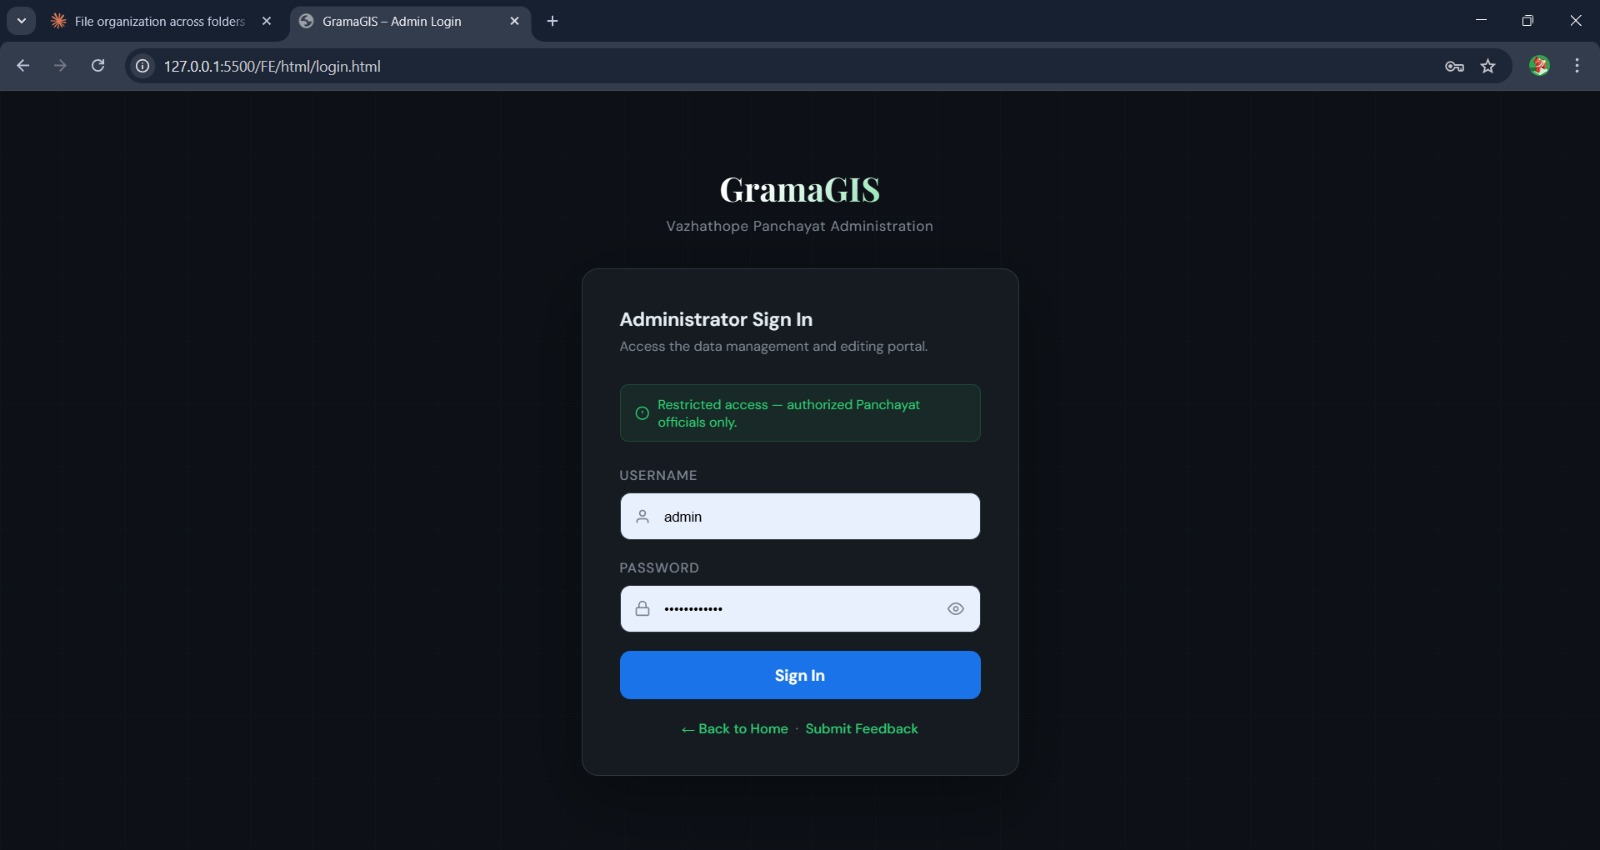
\includegraphics[width=0.85\textwidth]{Project_Screenshots/admin_login.jpeg}
    \caption{Secure administrator authentication interface with role-based access control}
    \label{fig:admin_login}
\end{figure}

Figure \ref{fig:admin_login} presents the secure login interface that restricts administrative functions to authorized Panchayat officials. The system implements JWT-based authentication to ensure that only verified users can access the transactional GIS (T-GIS) module for data editing and management.

\subsection{Data Management Interface}

\begin{figure}[H]
    \centering
    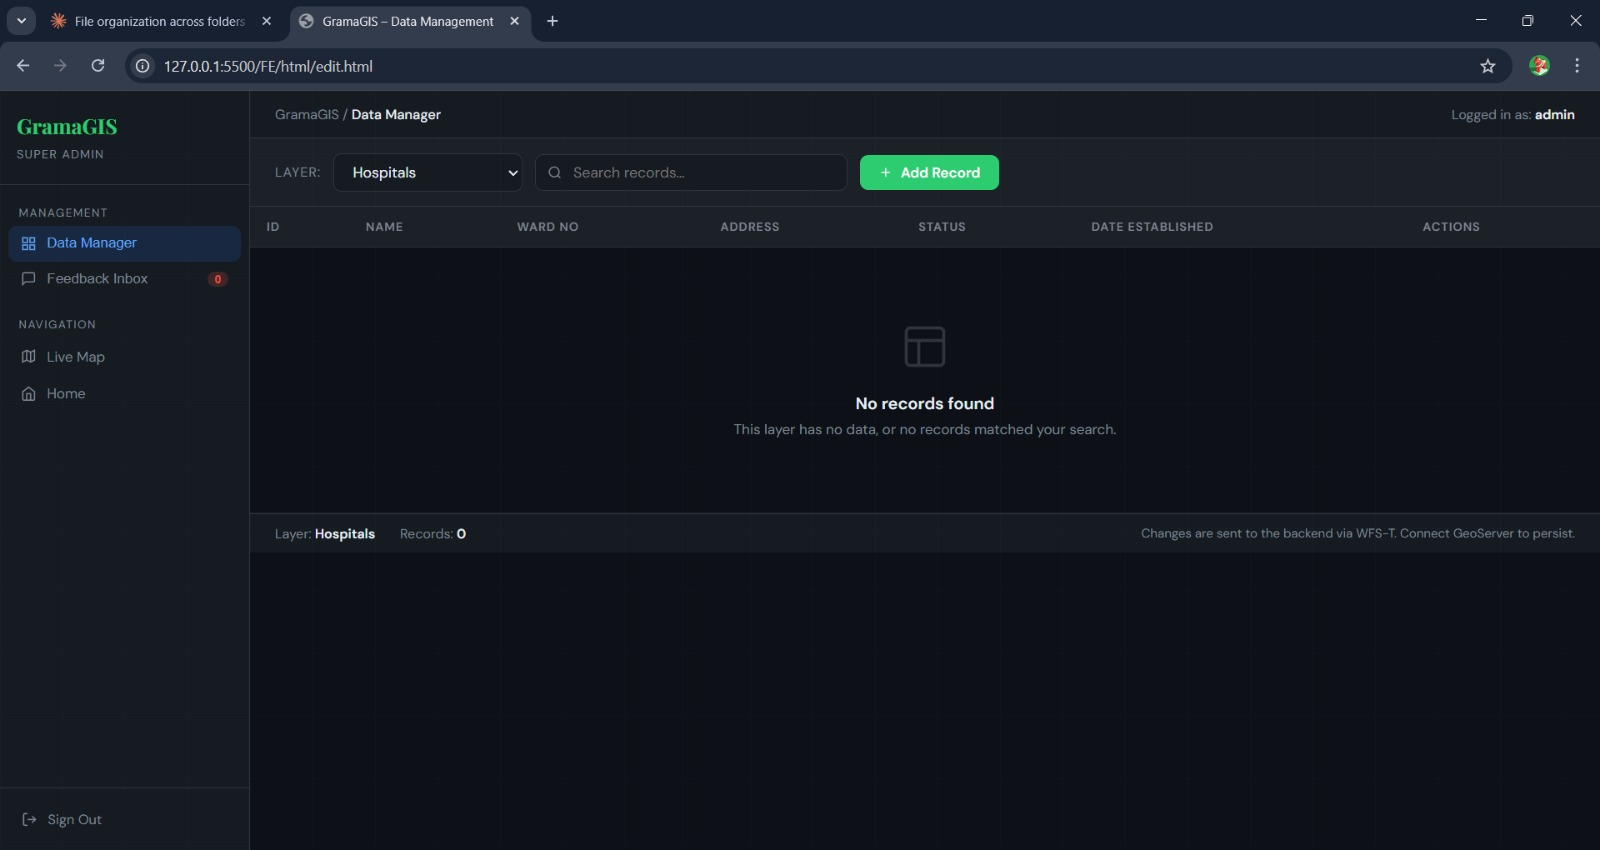
\includegraphics[width=0.85\textwidth]{Project_Screenshots/edit.jpeg}
    \caption{Administrative data management interface for updating infrastructure records}
    \label{fig:data_management}
\end{figure}

Figure \ref{fig:data_management} showcases the T-GIS module where administrators can add, edit, or delete infrastructure records. The interface provides a tabular view of all assets within a selected layer (e.g., hospitals, schools), allowing officials to update attributes such as name, ward number, address, and operational status. Changes are immediately committed to the PostGIS database via WFS-T transactions.

\subsection{Citizen Feedback System}

\begin{figure}[H]
    \centering
    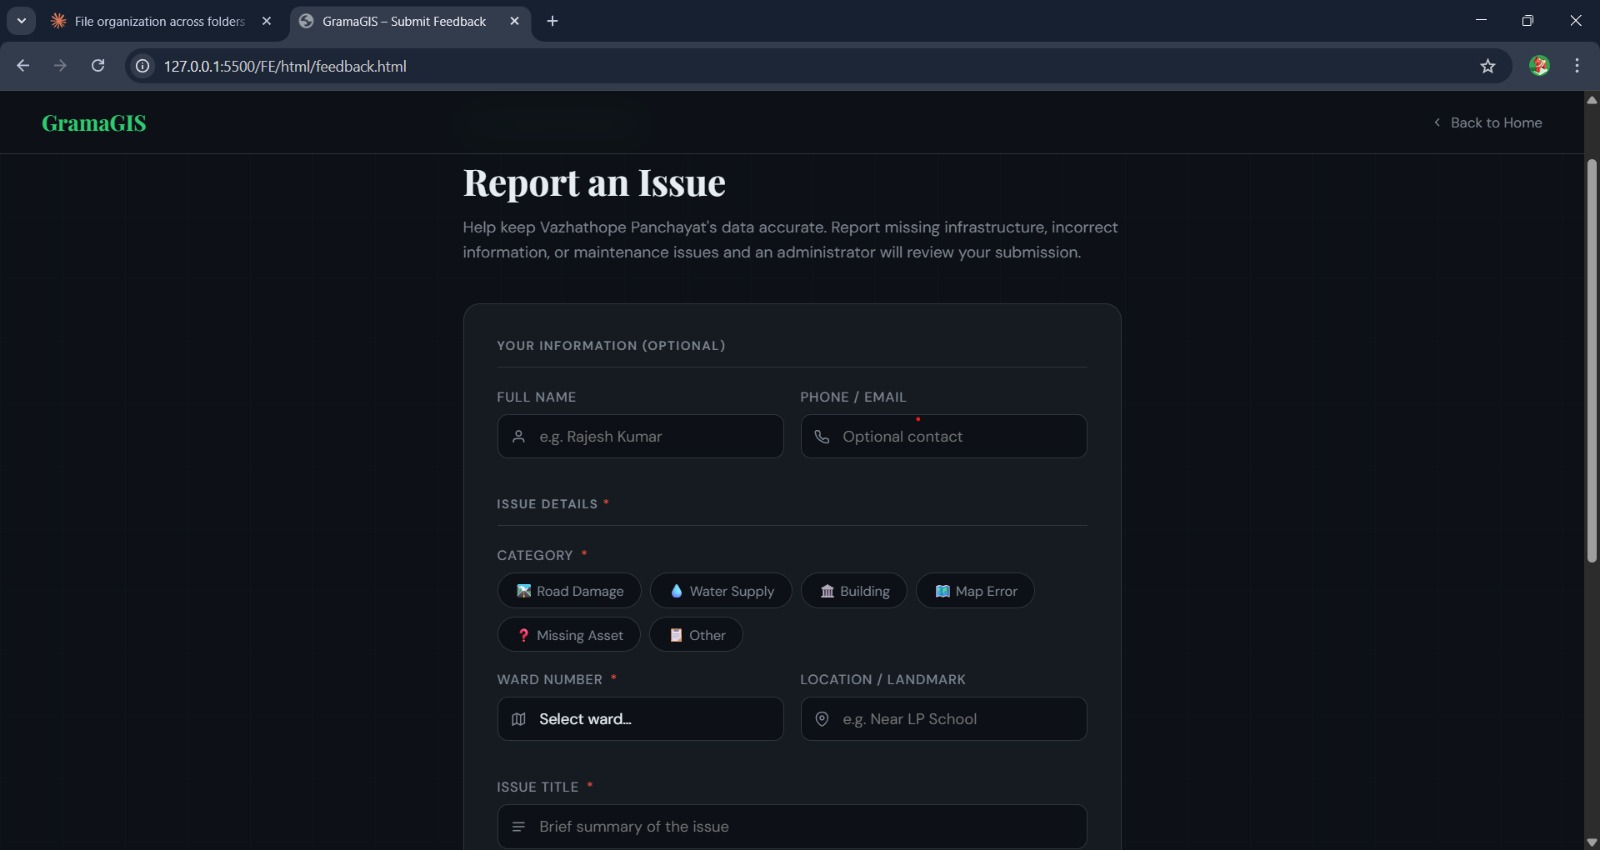
\includegraphics[width=0.85\textwidth]{Project_Screenshots/feedback.jpeg}
    \caption{Public feedback submission form for reporting infrastructure issues}
    \label{fig:feedback_form}
\end{figure}

Figure \ref{fig:feedback_form} illustrates the crowdsourced data validation system. Citizens can report missing infrastructure, incorrect information, or maintenance issues directly through the portal. The feedback is categorized by issue type (road damage, water supply, building, map error, missing asset) and linked to specific ward locations, enabling administrators to maintain an accurate and up-to-date village database.

\end{spacing}